\documentclass[12pt]{article}
\usepackage[spanish]{babel}
\usepackage{geometry}
\geometry{a4paper, margin=1in}
\usepackage{graphicx}
\usepackage{xcolor}
\usepackage{titlesec}
\usepackage{parskip}
\usepackage{multicol}
\usepackage{cite}
\usepackage{float}
\usepackage{listings}

\definecolor{highlight}{RGB}{255, 255, 0}

\titleformat{\section}{\normalfont\Large\bfseries}{\thesection}{1em}{}
\titleformat{\subsection}{\normalfont\large\bfseries}{\thesubsection}{1em}{}



\begin{document}

% Logos
\begin{minipage}{0.45\textwidth}
    
\includegraphics[width=0.4\textwidth]{inFiles/Figures/epnLogo.jpg}
\end{minipage}
\hfill
\begin{minipage}{0.45\textwidth}
    \raggedleft
    
\includegraphics[width=0.4\textwidth]{inFiles/Figures/FIS_logo.jpg}
\end{minipage}


\vspace{0.5cm}

% Títulos principales
\begin{center}
    \textbf{ESCUELA POLITÉCNICA NACIONAL}\\[0.2cm]
    \textbf{FACULTAD DE INGENIERÍA DE SISTEMAS}\\[0.2cm]
    \textbf{INGENIERÍA {\textbf{EN COMPUTACIÓN}}}
\end{center}

\vspace{0.5cm}
\hrule
\vspace{0.5cm}

% Datos principales
\noindent\textbf{PERÍODO ACADÉMICO:} 2025-A\\[0.2cm]
\noindent\textbf{ASIGNATURA:} ICCD412 Métodos Numéricos \hfill \textbf{GRUPO:} GR2\\[0.2cm]
\noindent\textbf{TIPO DE INSTRUMENTO:} Repaso 1\\[0.2cm]
\noindent\textbf{FECHA DE ENTREGA LÍMITE:} 15/06/2025\\[0.2cm]
\noindent\textbf{ALUMNO:} Murillo Tobar Juan

\vspace{0.5cm}
\hrule
\vspace{1cm}


% Secciones
\section{TEMA}
Repaso 1

\vspace{0.5cm}

\section{DESARROLLO}

\textbf{1. Calcule los diferentes tipos de errores en las aproximaciones de p por  p*, tome en cuenta 2 cifras significativas, 2 cifras por redondeo y 2 cifras por truncamiento.} 

\begin{figure}[H]
\centering
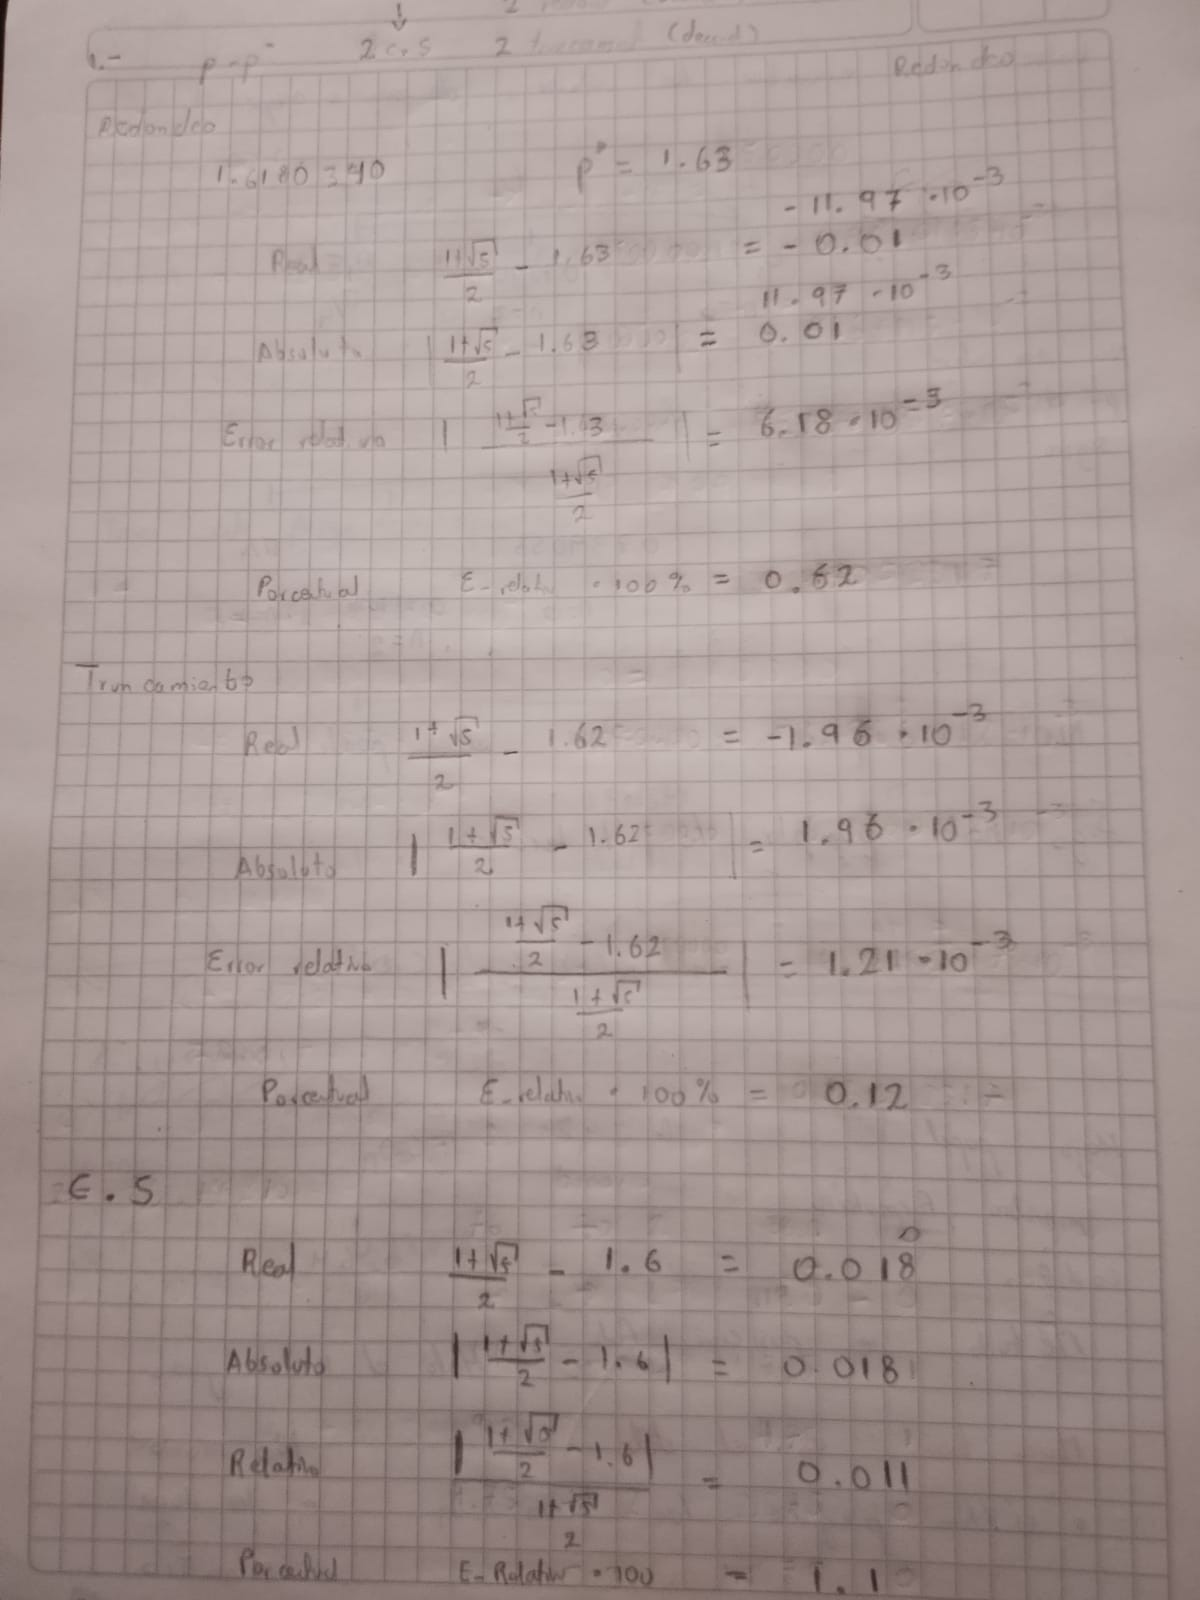
\includegraphics[width=1\textwidth]{./inFiles/Figures/11.jpeg}
\end{figure}

\textbf{2. Pasar 76.14810 al formato IEEE 754 de 32 bits.} 

\begin{figure}[H]
\centering
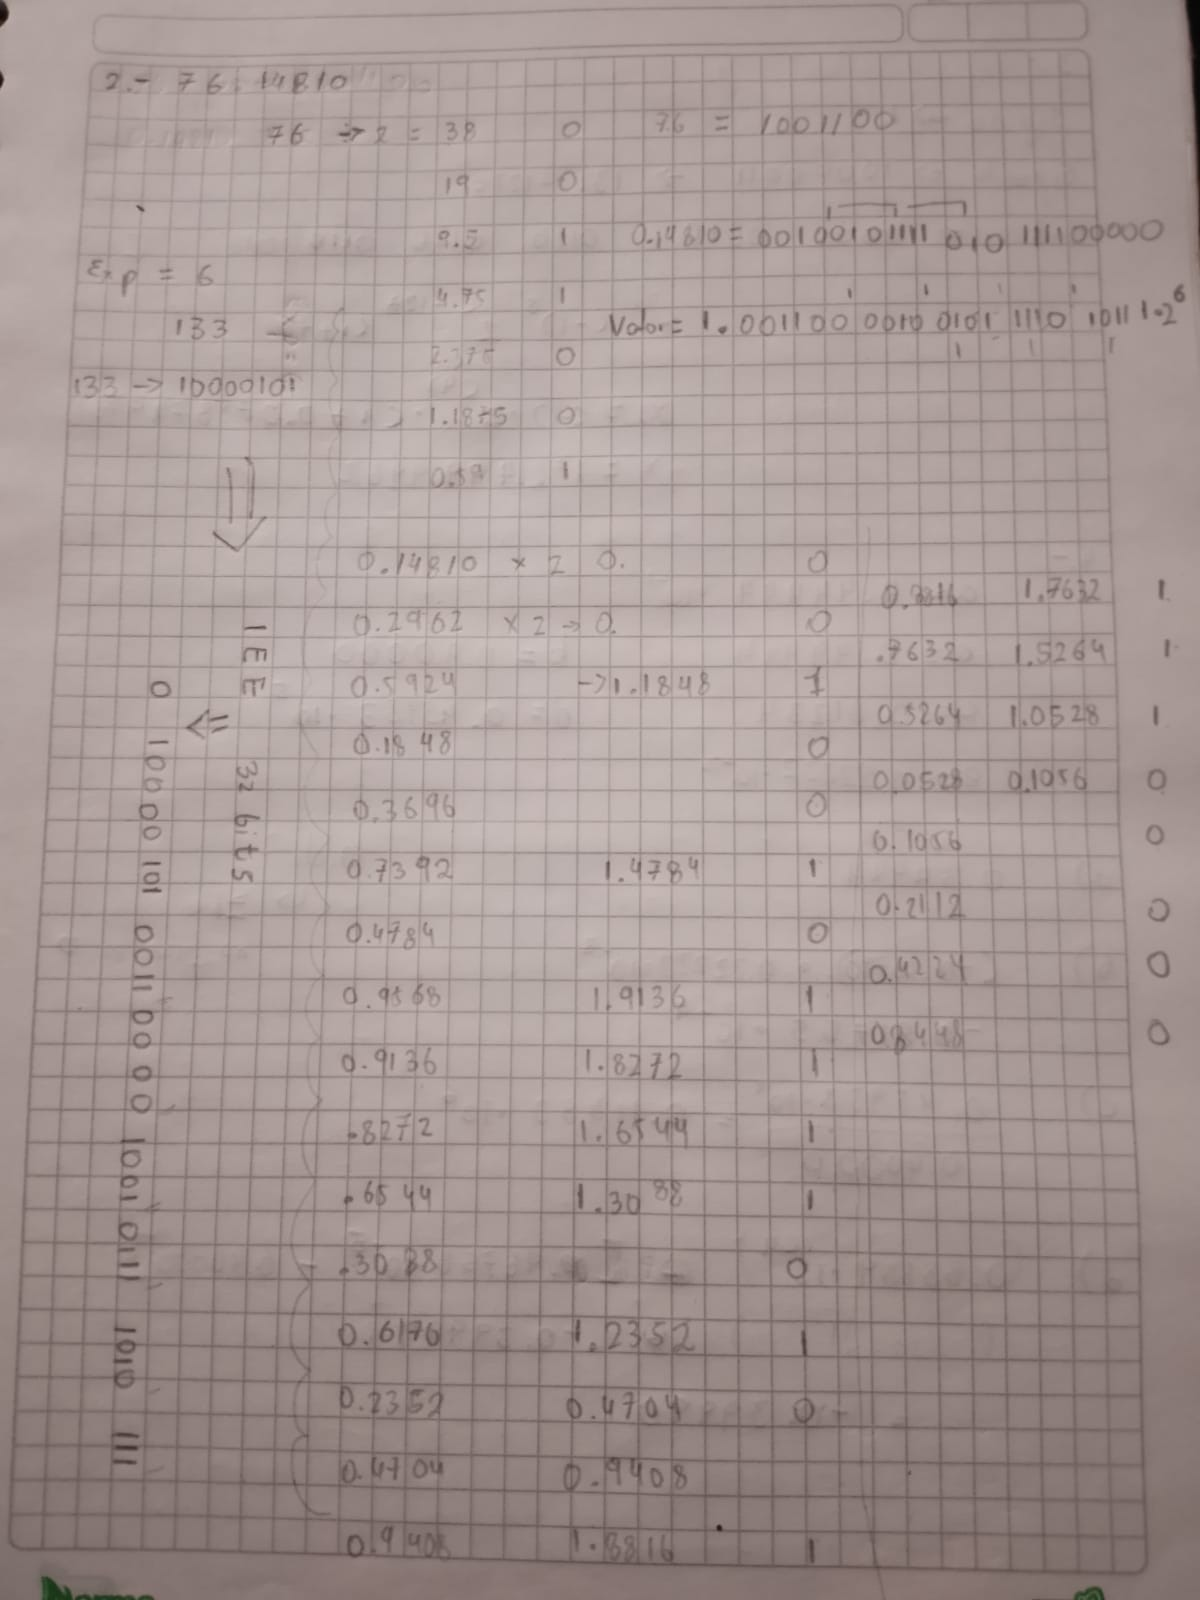
\includegraphics[width=1\textwidth]{./inFiles/Figures/10.jpeg}
\end{figure}

\textbf{3. Pasar de formato IEEE 754 11000001100010010011001100110011 a decimal.} 

\textbf{4. Suponga que $a = \frac{4}{9}$,  $b = \frac{2}{5}$, $c = 0.81234$, $d = 45932.7$, $e = 0.22222*10^{-3}$ resuelva con 5 cifras con redondeo}

\begin{figure}[H]
\centering
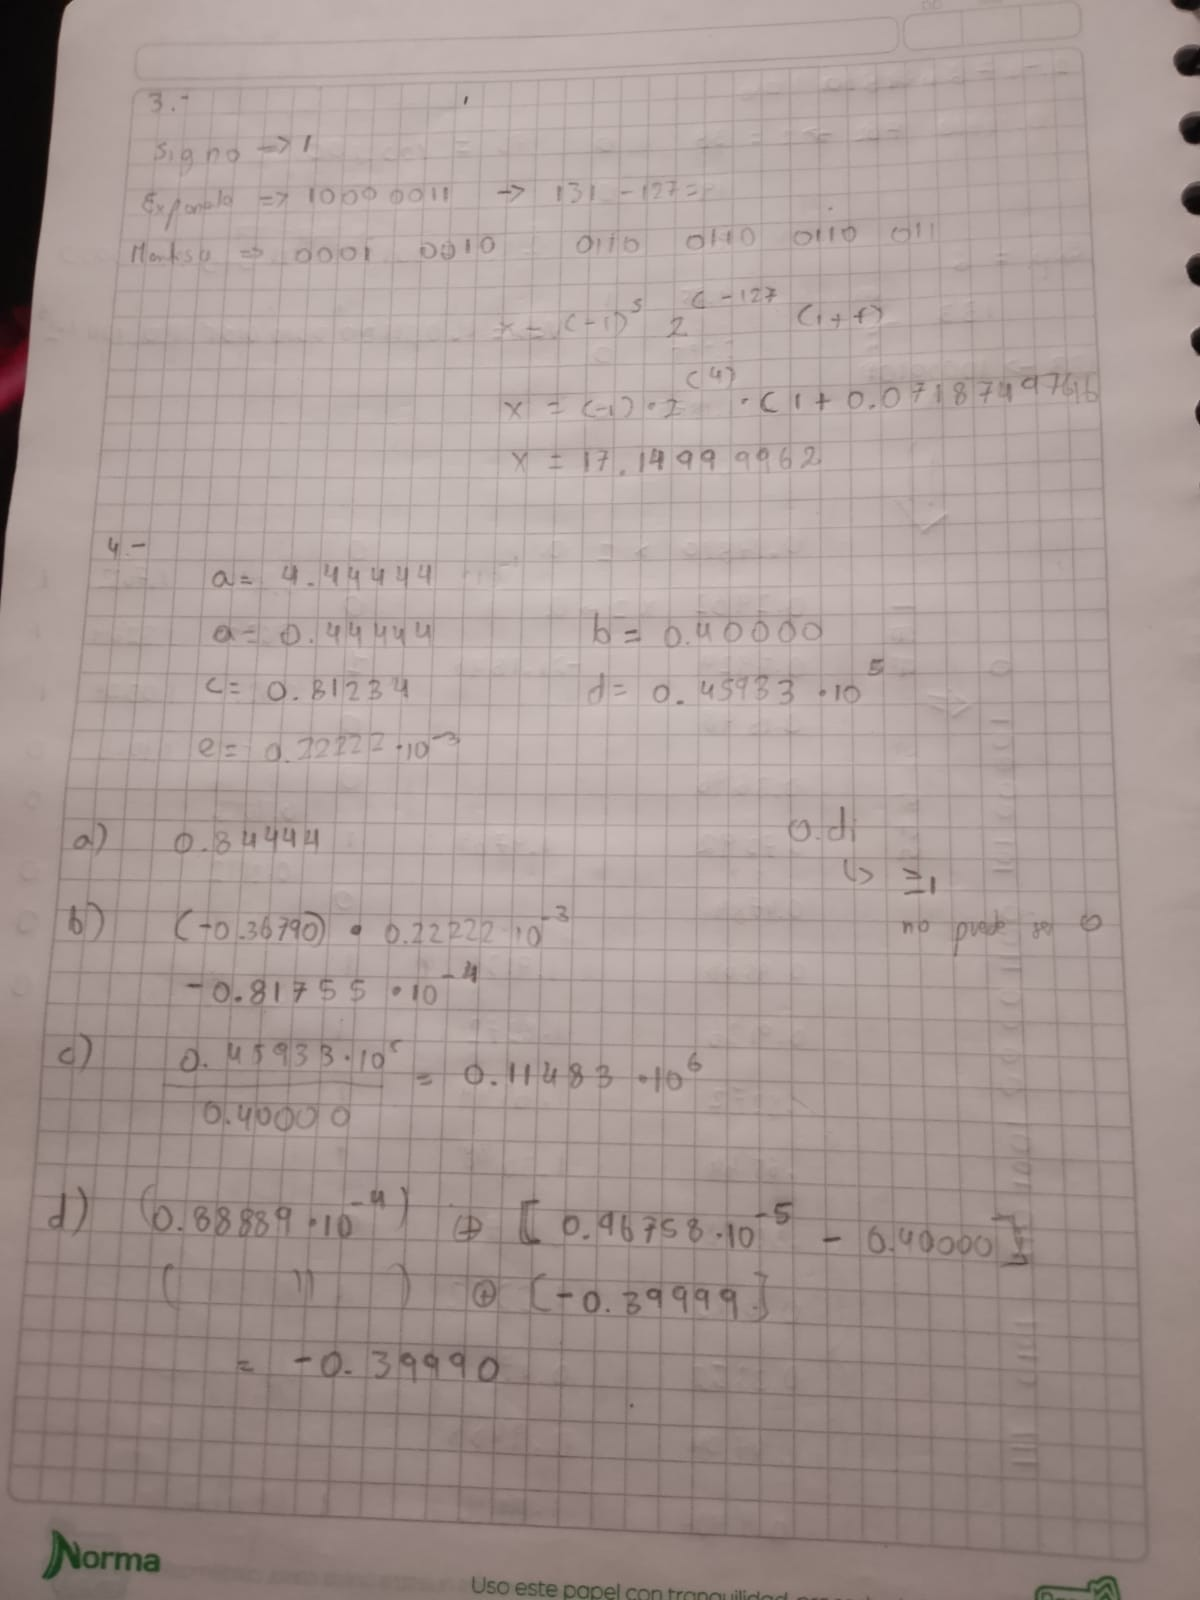
\includegraphics[width=1\textwidth]{./inFiles/Figures/9.jpeg}
\end{figure}

\textbf{5. Dada la función $f(x) = x^4 - x - 1$, use método de la bisección para los intervalos [-1;0] y [1,2], obtener soluciones precisas dentro de $10^{-6}$ como tolerancia, trabaje con 8 cifras decimales por redondeo. Muestre tabla de valores.} 

Primer intervalo
\begin{figure}[H]
\centering
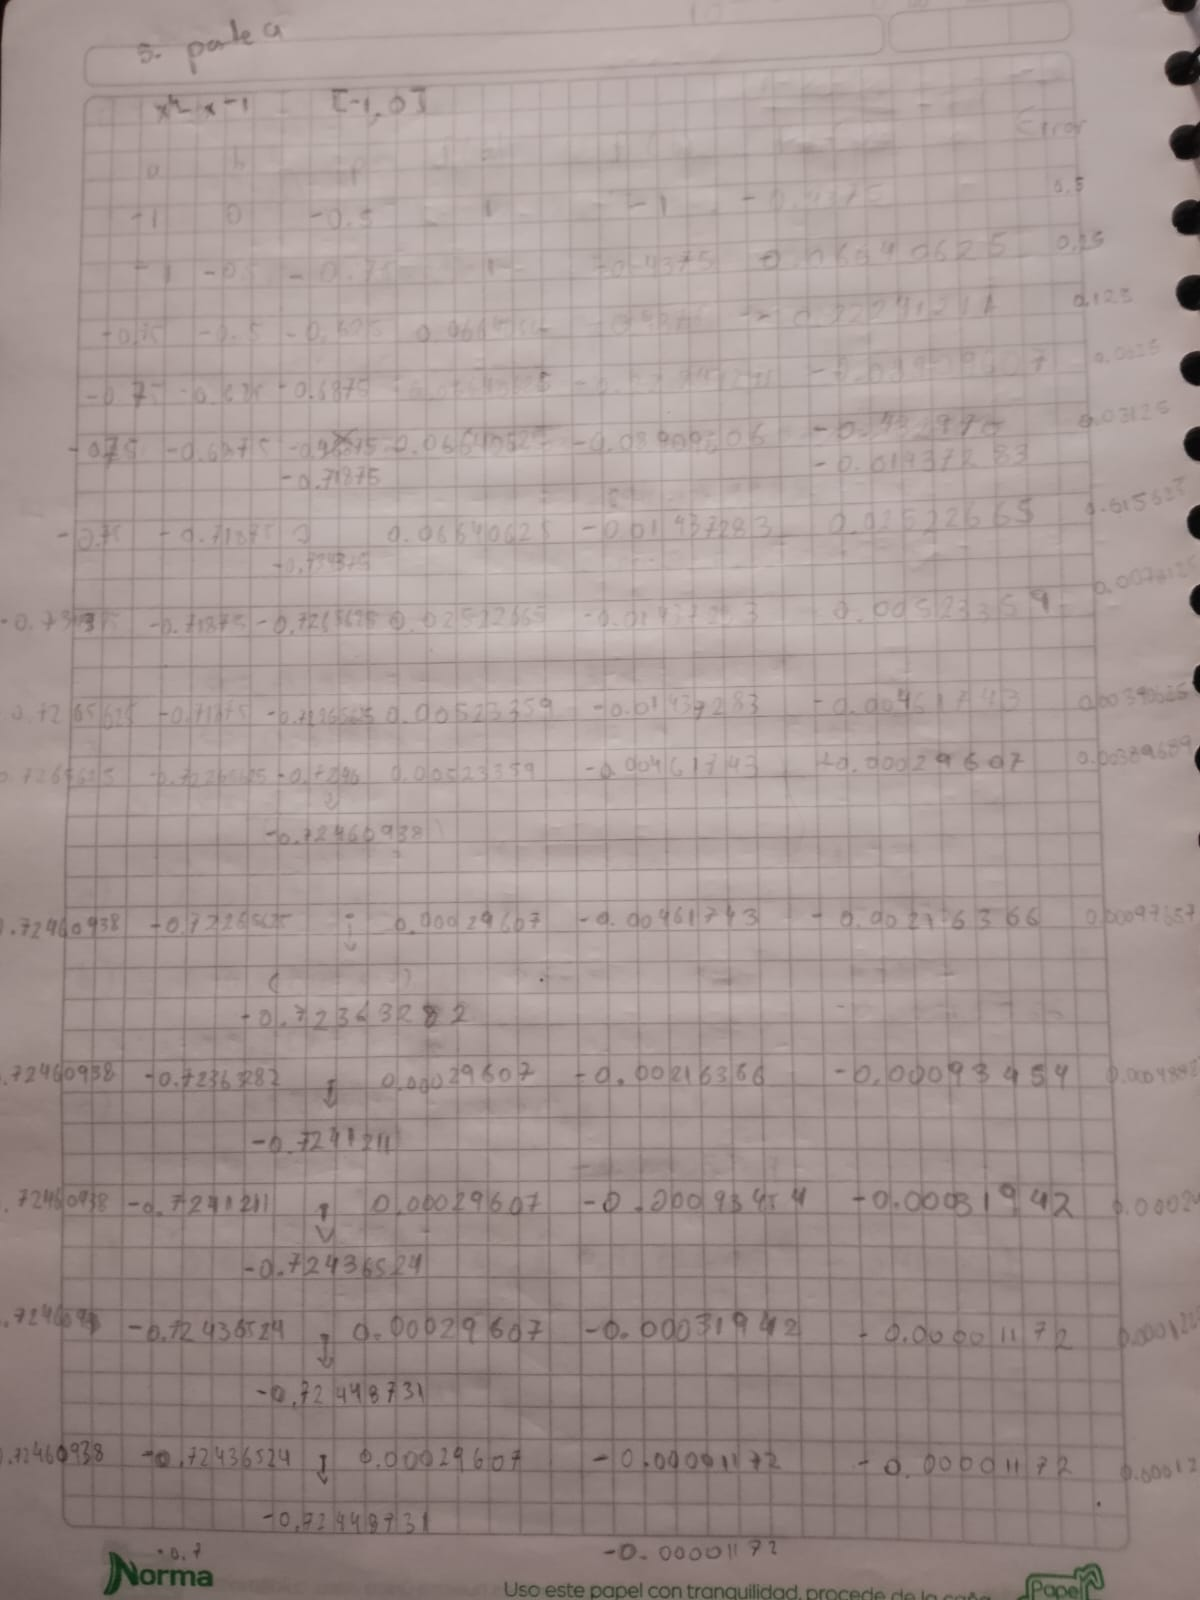
\includegraphics[width=1\textwidth]{./inFiles/Figures/8.jpeg}
\end{figure}

\begin{figure}[H]
\centering
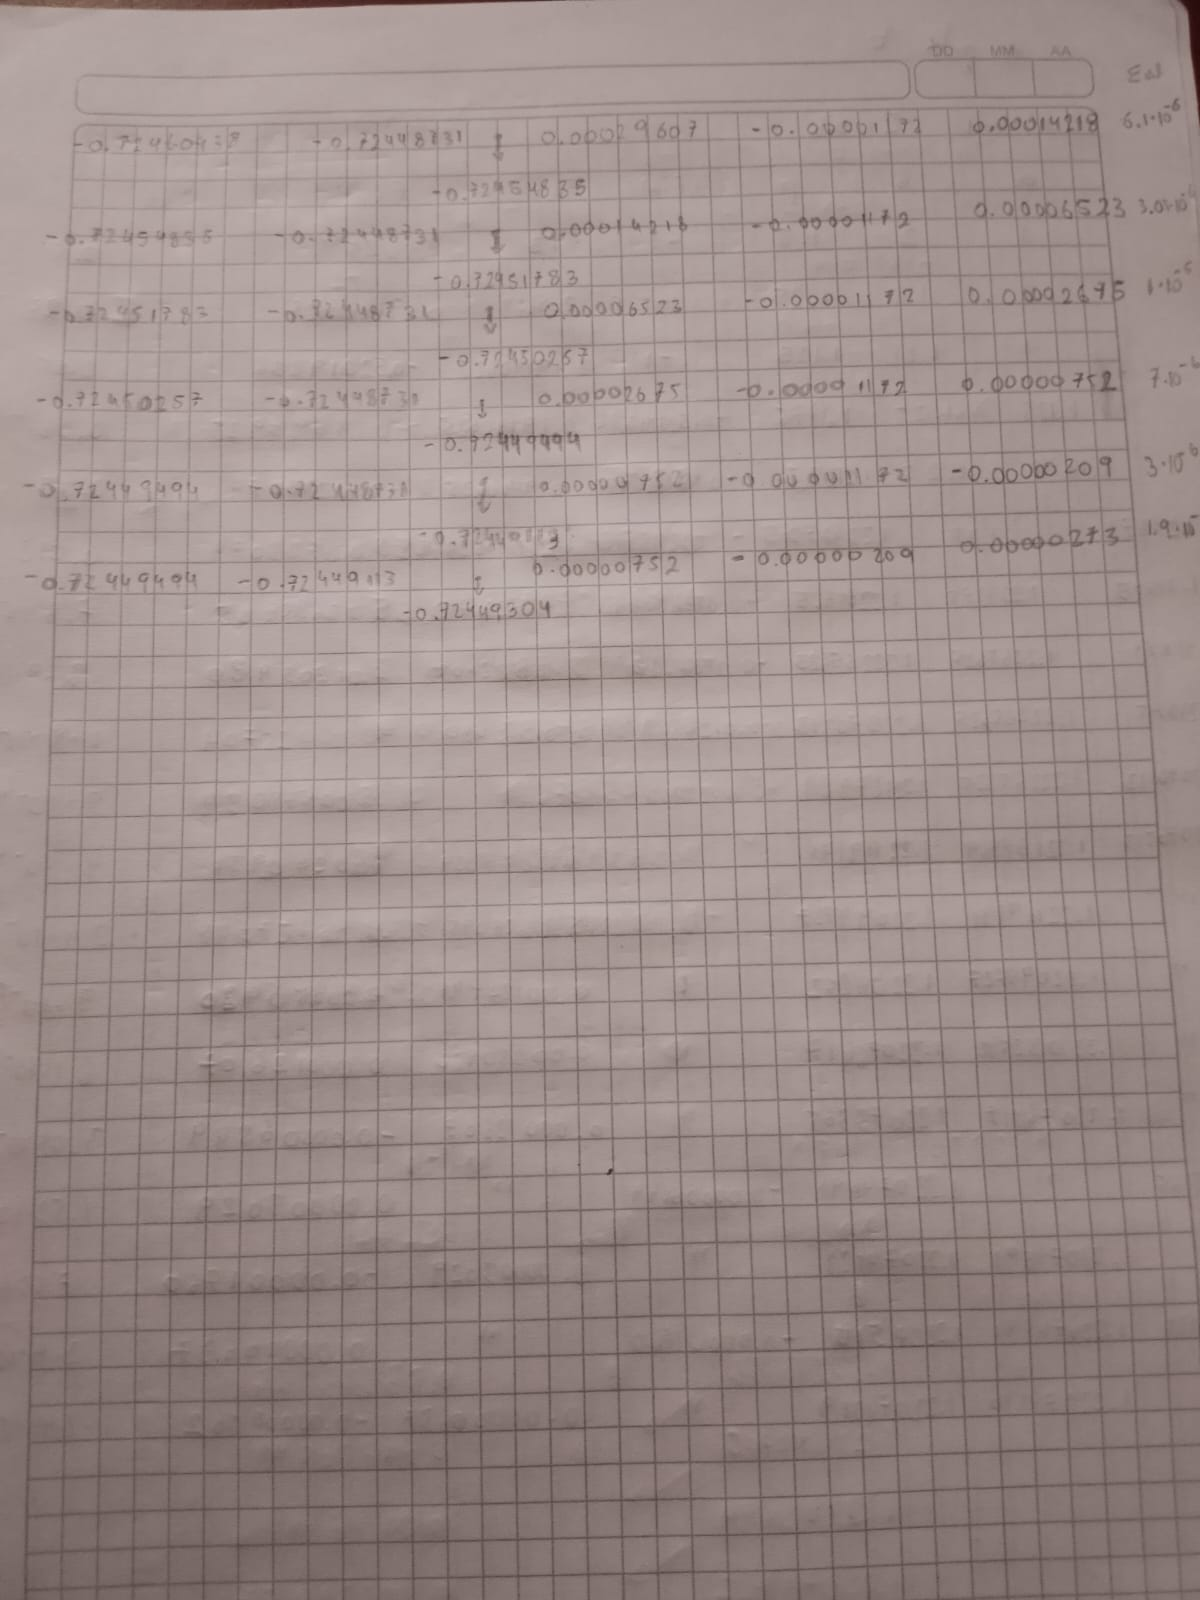
\includegraphics[width=1\textwidth]{./inFiles/Figures/7.jpeg}
\end{figure}

Segundo intervalo
\begin{figure}[H]
\centering
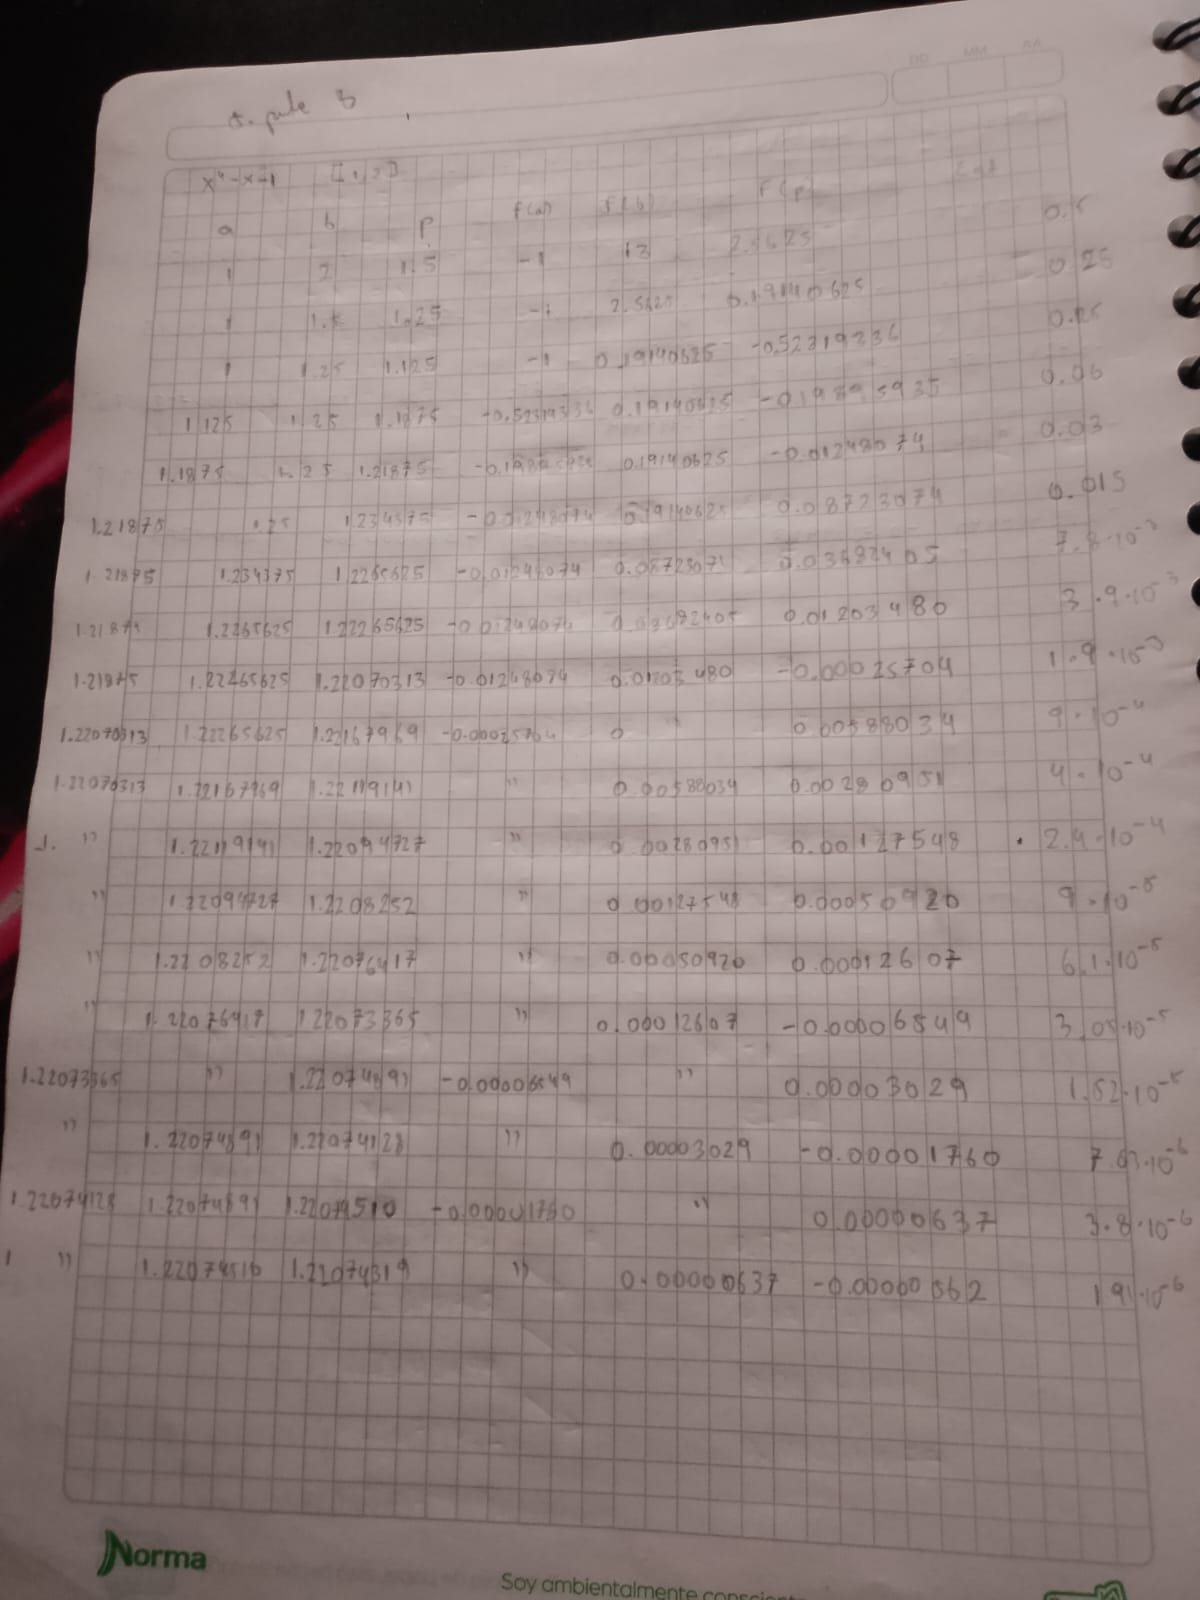
\includegraphics[width=1\textwidth]{./inFiles/Figures/6.jpeg}
\end{figure}



\textbf{6. Dada la función $f(x) = x^4 + 4x^2 - 10$, determine el número de iteraciones necesarias con precisión $10^{-5}$, a = 1 y b = 2, trabaje con 8 cifras significativas} 


\begin{figure}[H]
\centering
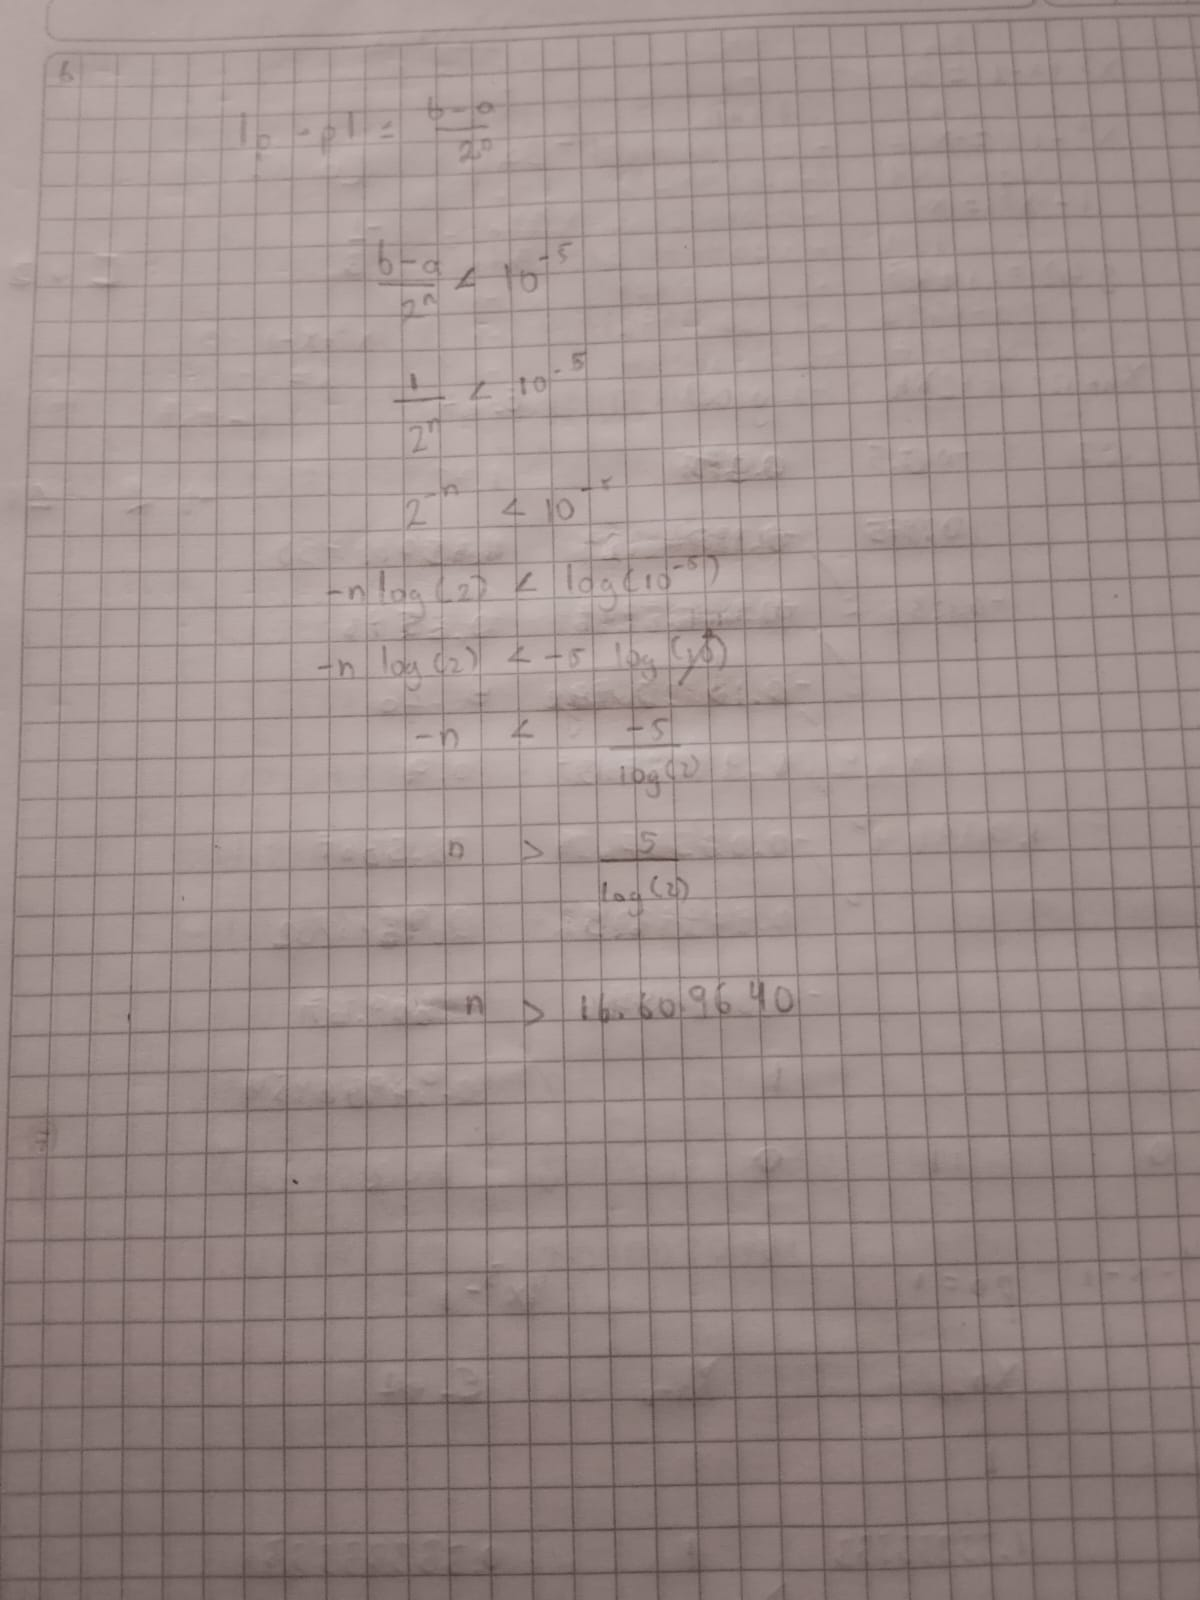
\includegraphics[width=1\textwidth]{./inFiles/Figures/5.jpeg}
\end{figure}





\textbf{7. Dada la función $f(x) = \frac{x^3+x-1,}{3}$ use el método del punto fijo donde p se encuentra en (0;1), y obtenga soluciones precisas dentro de $10^{-3}$, trabaje con 8 cifras decimales por truncamiento. Muestre tabla de valores.} 


\begin{figure}[H]
\centering
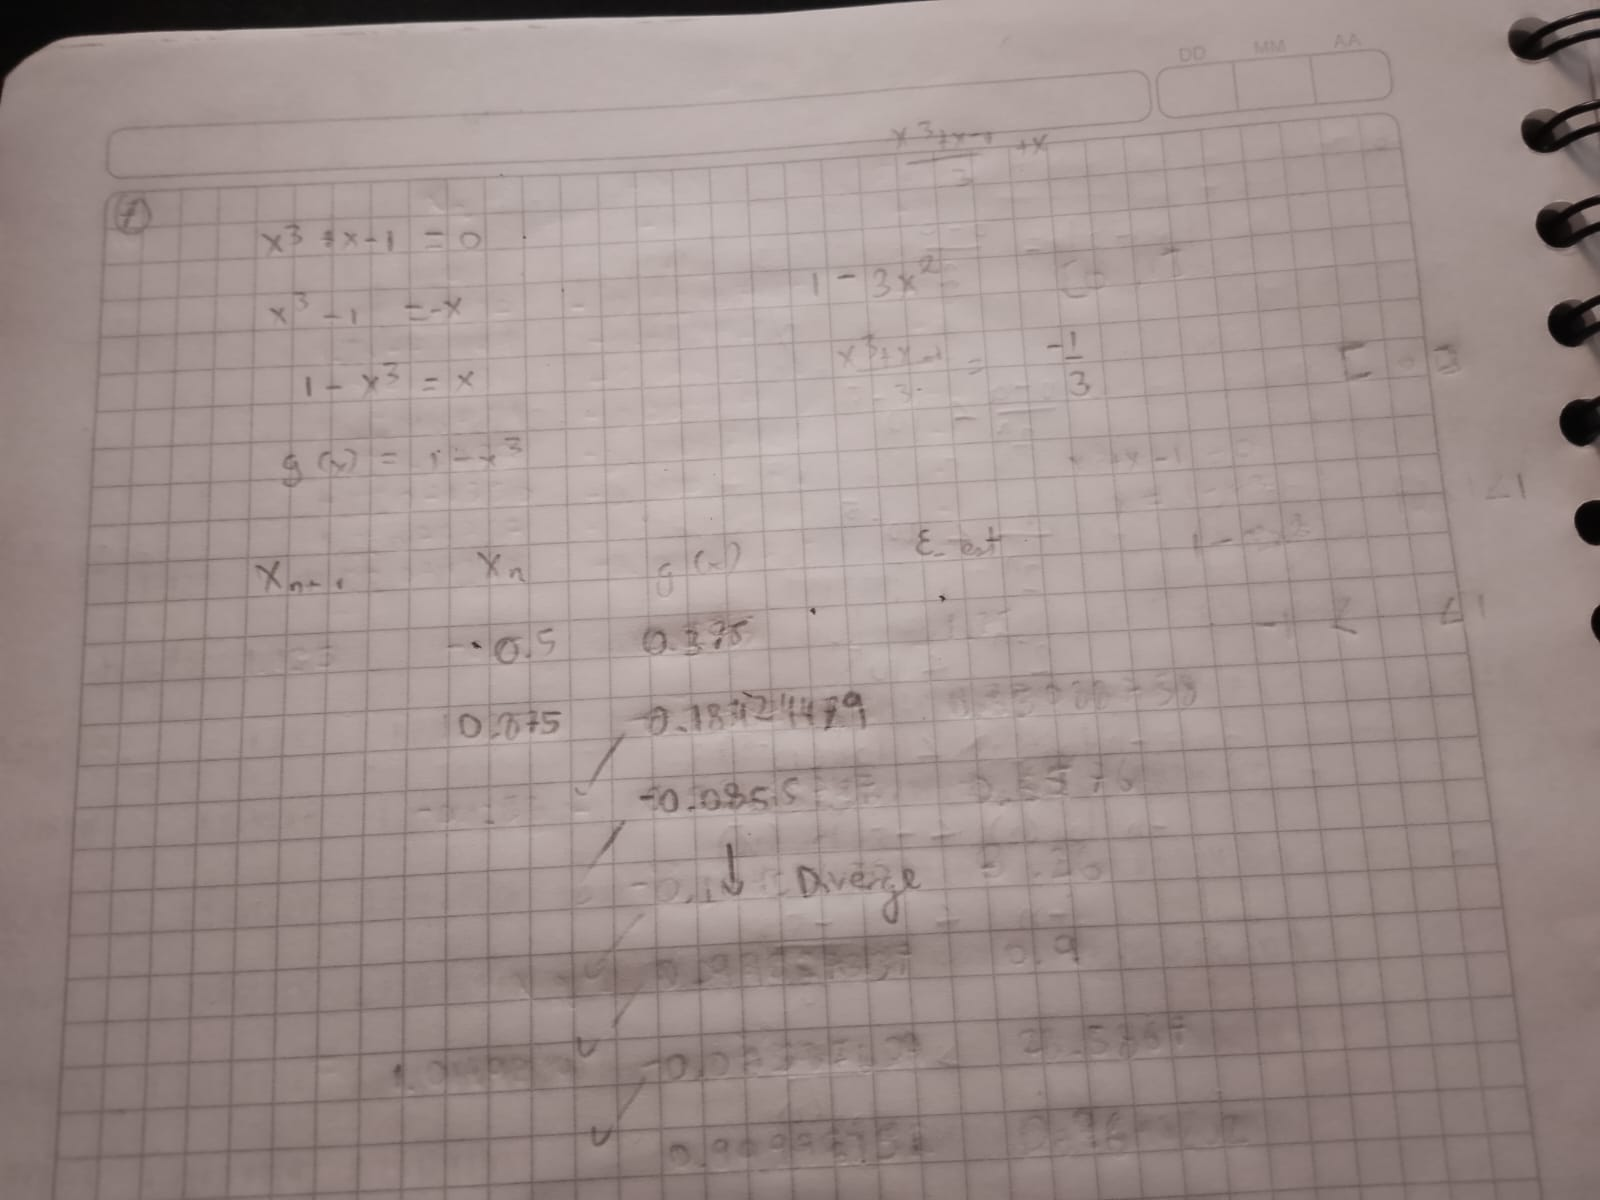
\includegraphics[width=1\textwidth]{./inFiles/Figures/4.jpeg}
\end{figure}




\textbf{8. Dada la función $f(x) = x^4-x- 1$, p0 = 1, use el método de Newton obtener soluciones precisas con tolerancia $10^{-6}$, trabaje con 8 cifras decimales por truncamiento. Muestre tabla de valores.} 

\begin{figure}[H]
\centering
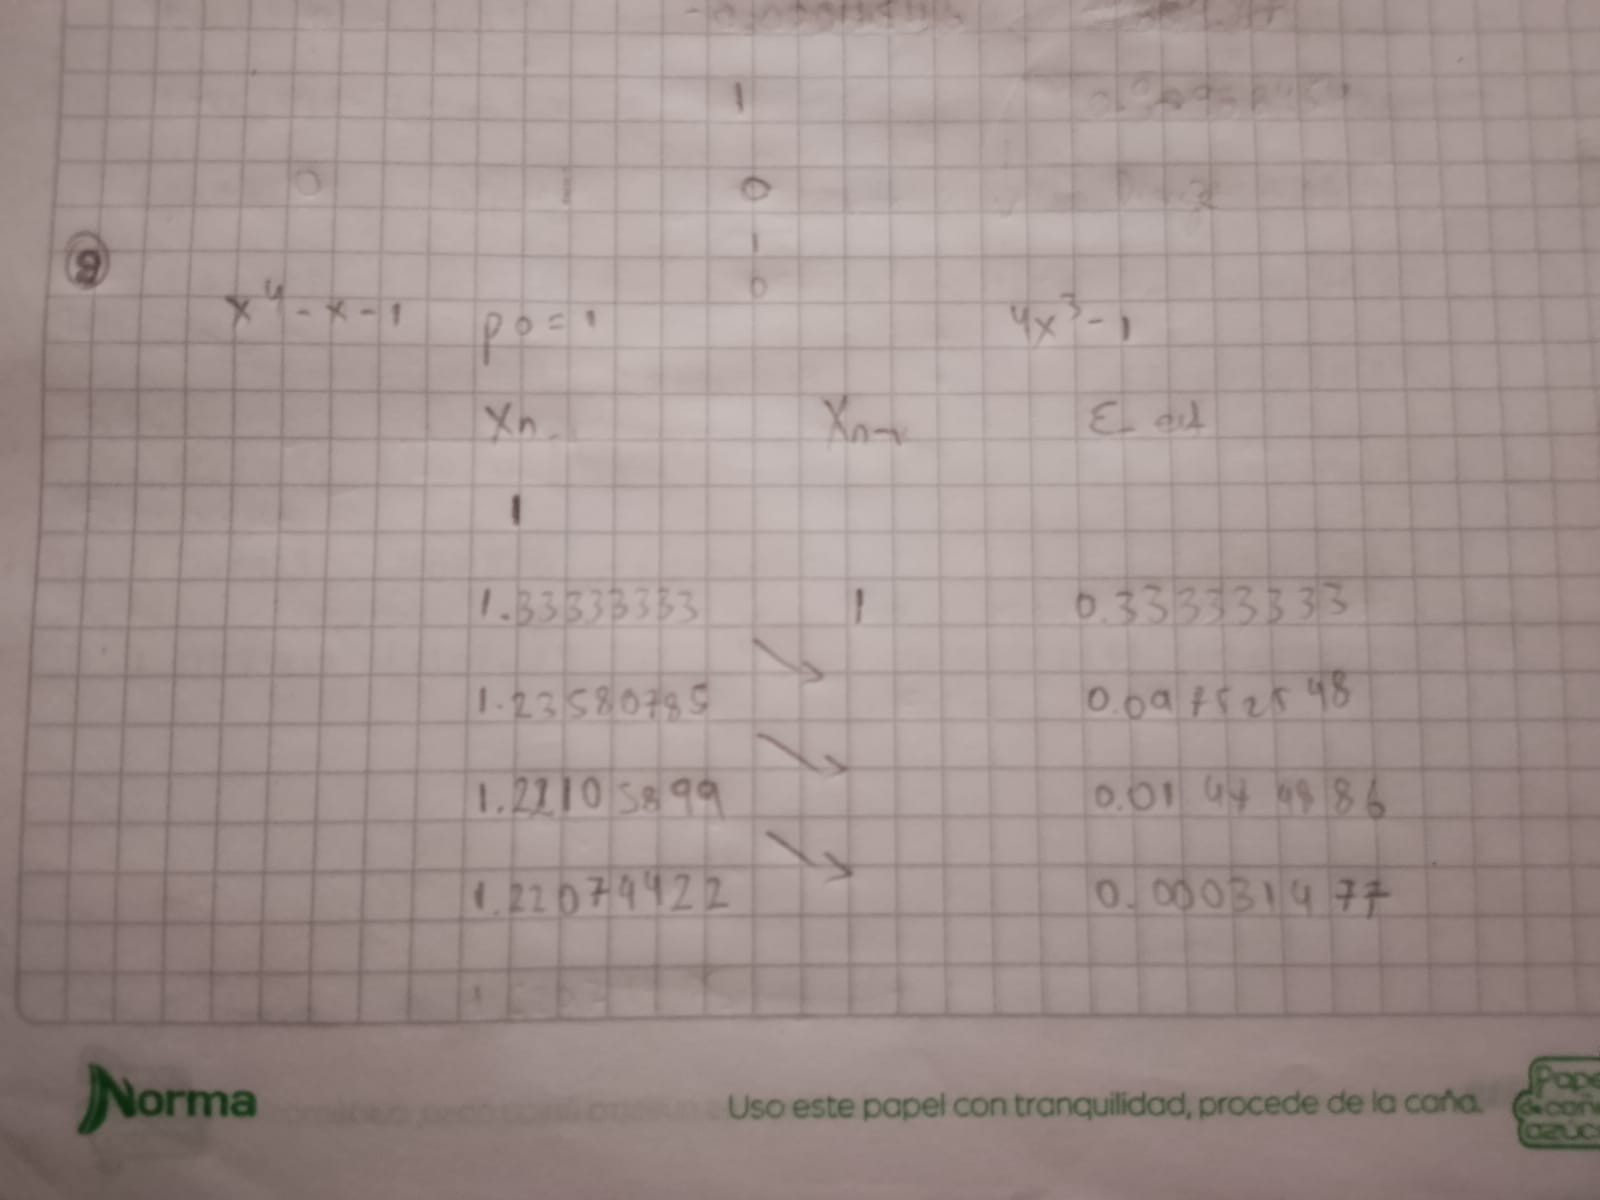
\includegraphics[width=1\textwidth]{./inFiles/Figures/3.jpeg}
\end{figure}




\textbf{9. Dada la función $f(x) = x^4-x- 1$, p0 = 1 y p1 = 1.4, use el método de la Secante, obtener soluciones precisas con tolerancia $10^{-6}$, trabaje con 8 cifras decimales por truncamiento. Muestre tabla de valores.} 


\begin{figure}[H]
\centering
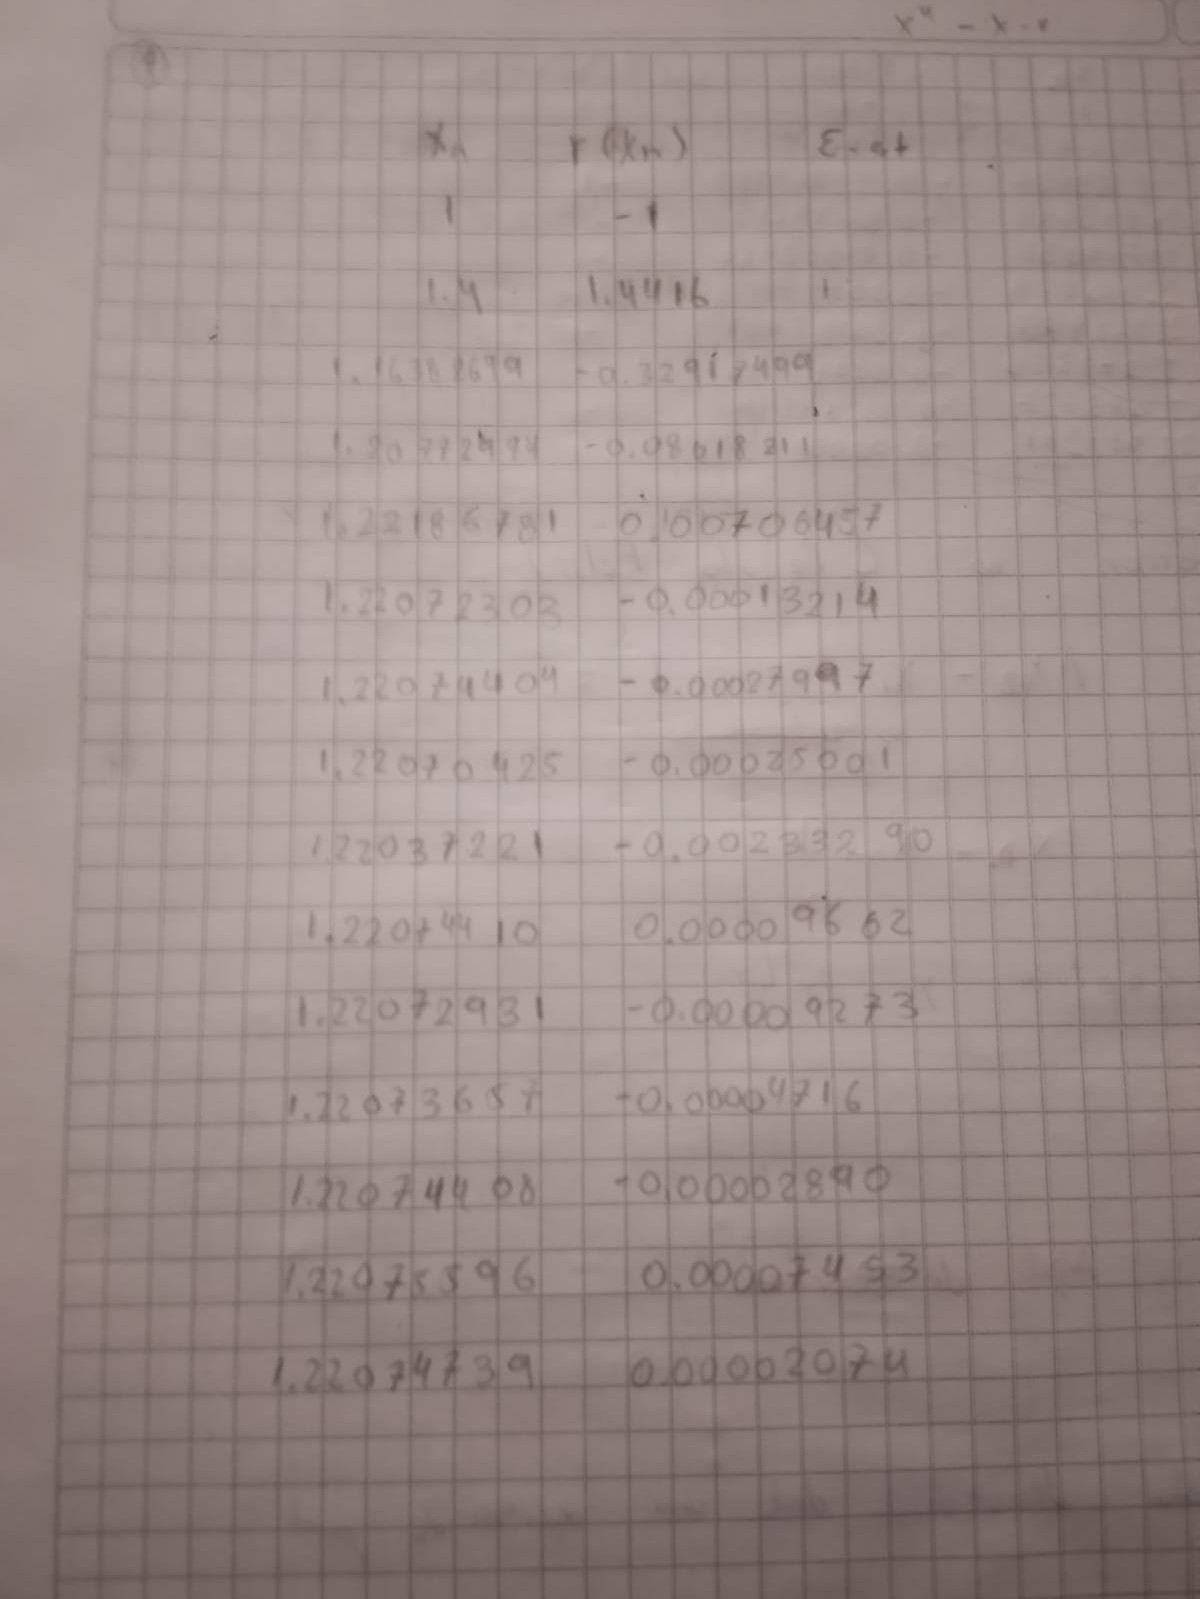
\includegraphics[width=1\textwidth]{./inFiles/Figures/2.jpeg}
\end{figure}



\textbf{10. Dada la función $f(x) = x^4-x- 1$, p0 = 1 y p1 = 1.4, use el método de la Posición Falsa, obtener soluciones precisas con tolerancia $10^{-6}$, trabaje con 8 cifras decimales por redondeo. Muestre tabla de valores.} 

\begin{figure}[H]
\centering
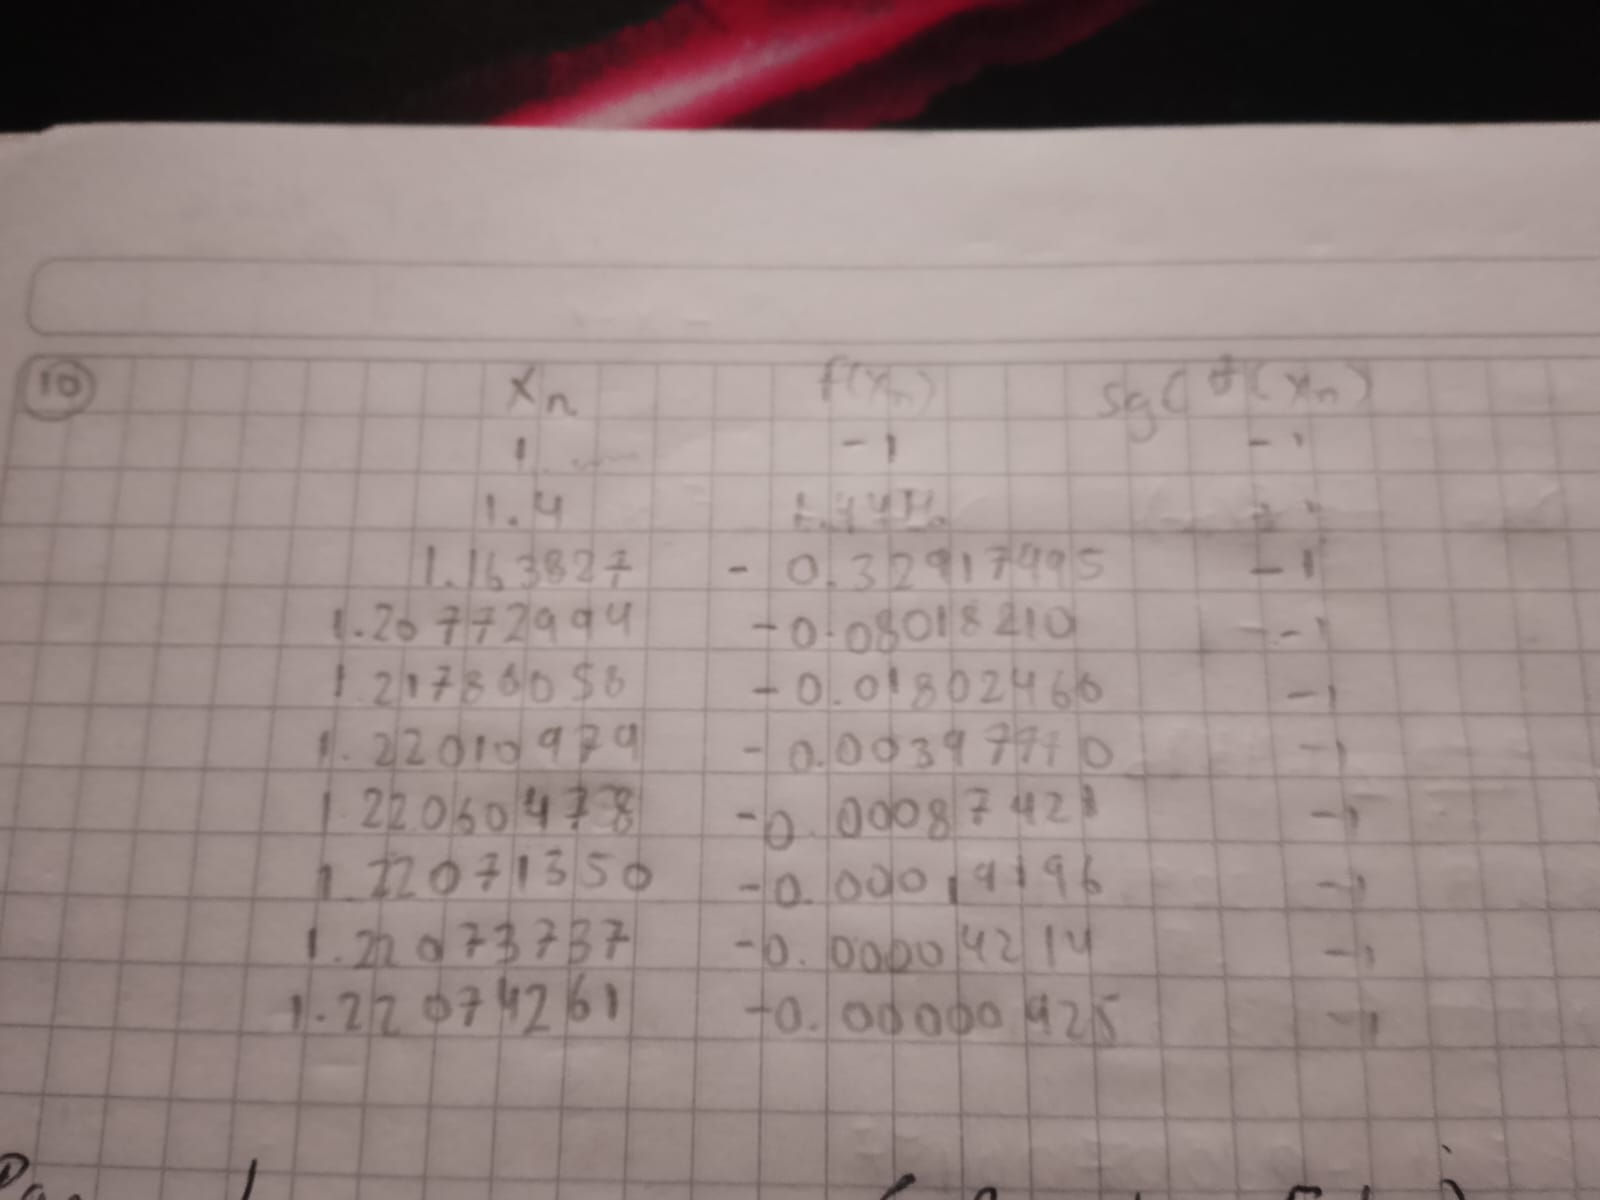
\includegraphics[width=1\textwidth]{./inFiles/Figures/1.jpeg}
\end{figure}



\textbf{11. Dada la función $f(x) = x^4-x- 1$, justifique cual es mejor } 

El mejor es el método de la posición falsa porque toma dos aproximaciones iniciales y es mucho mas rápida que el de la bisección. Sumado a estos, ambos métodos son cerrados por lo que van a converger y ademas no necesitan de cálculos complicados 
como lo es el método de Newton 

\vspace{0.5cm}


\end{document}
